% !TEX root = ../../../main.tex
% 来源：中学数学实验教材·第二册（几何）
% 章节：三角比与角边关系 / 解直角三角形
% 原始文件：6.tex，行 1133-1144
% 类型：tikz
% ---
    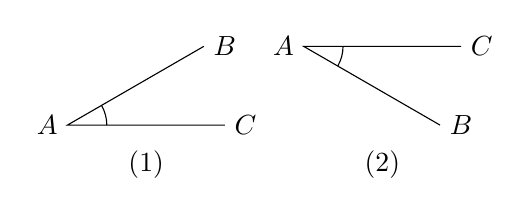
\begin{tikzpicture}[>=latex, scale=1]
\begin{scope}
\draw(30:2)node[right]{$B$}--(0,0)node[left]{$A$}--(2,0)node[right]{$C$};
\node at (1,-.5){(1)};
\draw(0.5,0) arc (0:30:.5);
\end{scope}
\begin{scope}[xshift=3cm]
    \draw(2,1)node[right]{$C$}--(0,1)node[left]{$A$}--+(-30:2)node[right]{$B$};
    \node at (1,-.5){(2)};
    \draw(0.5,1) arc (0:-30:.5);
\end{scope}
    \end{tikzpicture}
